\documentclass[letterpaper, 12pt]{article}
\usepackage[top=2cm,bottom=1cm,left=0.75in,right=0.75in,headheight=17pt, % as per the warning by fancyhdr
includehead,includefoot,
heightrounded, % to avoid spurious underfull messages
]{geometry}
\addtolength{\topmargin}{-.25in}
\usepackage{fancyhdr}
\pagestyle{fancy}
\usepackage{graphicx}
\usepackage{lastpage}
\usepackage{gensymb}

\begin{document}
\fancyhead[l]{	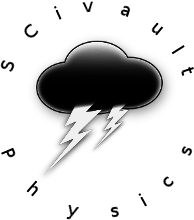
\includegraphics[height=1.2cm]{../Logo/sp.png} Name:}
\fancyhead[r]{REFERENCE MATERIAL}
\cfoot{\thepage\ of \pageref{LastPage}}
	


\begin{center}Things to Memorize: Circular Motion and Orbits
\end{center}

\subsection*{Centripetal Force and Acceleration}
	\begin{itemize}
		\item Any force that causes an object to move in a circle is a \textbf{centripetal force}. 
		\item A centripetal force is always directed toward the center of the circle the object moves in. (The word \textit{centripetal} means ``center-seeking".)
	\end{itemize}
\subsection*{Kepler's Laws}
	\begin{enumerate}
		\item \textit{All planets move about the Sun in elliptical orbits, having the Sun as one of the foci.}
			\begin{itemize}
				\item The eccentricity determines how close to a circle an objects orbit is.  
				\begin{center}
					\begin{tabular}{|c|c|} \hline
						 \textbf{Shape} & \textbf{Eccentricity} \\ \hline
						  Circle & $\varepsilon = 0 $ \\ \hline
						  Elipse & $ 0 < \varepsilon  < 1 $ \\ \hline
						  Parabola & $\varepsilon = 1 $ \\ \hline
						  Hyperbola & $ \varepsilon  > 1 $ \\ \hline
						  
						 
					\end{tabular}
				\end{center}
				\item All 8 planets have very low eccentricity.  (For example,  $ \varepsilon_{Earth} = 0.0167086$)
				\item Some comets follow hyperbolic paths. 
			\end{itemize}
		
		\item\textit{ A radius vector joining any planet to the Sun sweeps out equal areas in equal lengths of time.}
		\begin{itemize}
			\item This means planets move faster when closer to the sun and slower when farther from the sun. 
		\end{itemize}
		
		\item \textit{The squares of the sidereal periods (of revolution) of the planets are directly proportional to the cubes of their mean distances from the Sun. }
		\begin{itemize}
			\item This law works for any set of objects that orbit the same central body.  So two planets, a planet and a comet, and even two moons of Jupiter will work.  It does NOT work when the two objects do not orbit the same central body.  
		\end{itemize}
		
	\end{enumerate}

\subsection*{Universal Gravitation}
	\begin{itemize}
		\item Universal Gravitation is used when you wish to find the force of gravity between two objects when they are separated by significant distances.  
	\end{itemize}

\subsection*{Orbital Motion}
	\begin{itemize}
		\item In order for an object to have a stable orbit, \textbf{gravity} must act as a \textbf{centripetal force}. 
		\item Combining Newton's Law of Universal Gravitation with centripetal force allows Kepler's 3rd Law to be derived.  
		\item Most orbital motion problems will require you to equate the formula for Universal Gravitation with the formula for centripetal force. 
		
		
	\end{itemize}

\subsection*{Angular Velocity and Acceleration}
Before Beginning this section, be sure to review the section on \textbf{Arc Length.} 

\begin{itemize}
	\item \textbf{Angular Velocity} measures how quickly something is rotating.  
	\begin{itemize}
		\item Units: rad/s
		\item Symbol: $\omega$
	\end{itemize}
	\item \textbf{Angular Acceleration} measure how quickly an object's angular velocity is changing (speeding up or slowing down).  
	\begin{itemize}
		\item Units: rad/s\textsuperscript{2}
		\item Symbol: $\alpha$
	\end{itemize}

\end{itemize}

\subsection*{Angular Kinematics}

\subsection*{Torque}

\subsection*{Angular Momentum}

 




\end{document}
